\section{Tree Types \& Traversals}

\subsection{Binary Trees: 2 Children}

\noindent
First we'll define a basic binary tree and then all its extensions.
\begin{Def}[Binary Tree]

    A \textbf{binary tree} is a tree where each parent node has at most two children.
\end{Def}

\begin{figure}[h]
    \begin{center}
    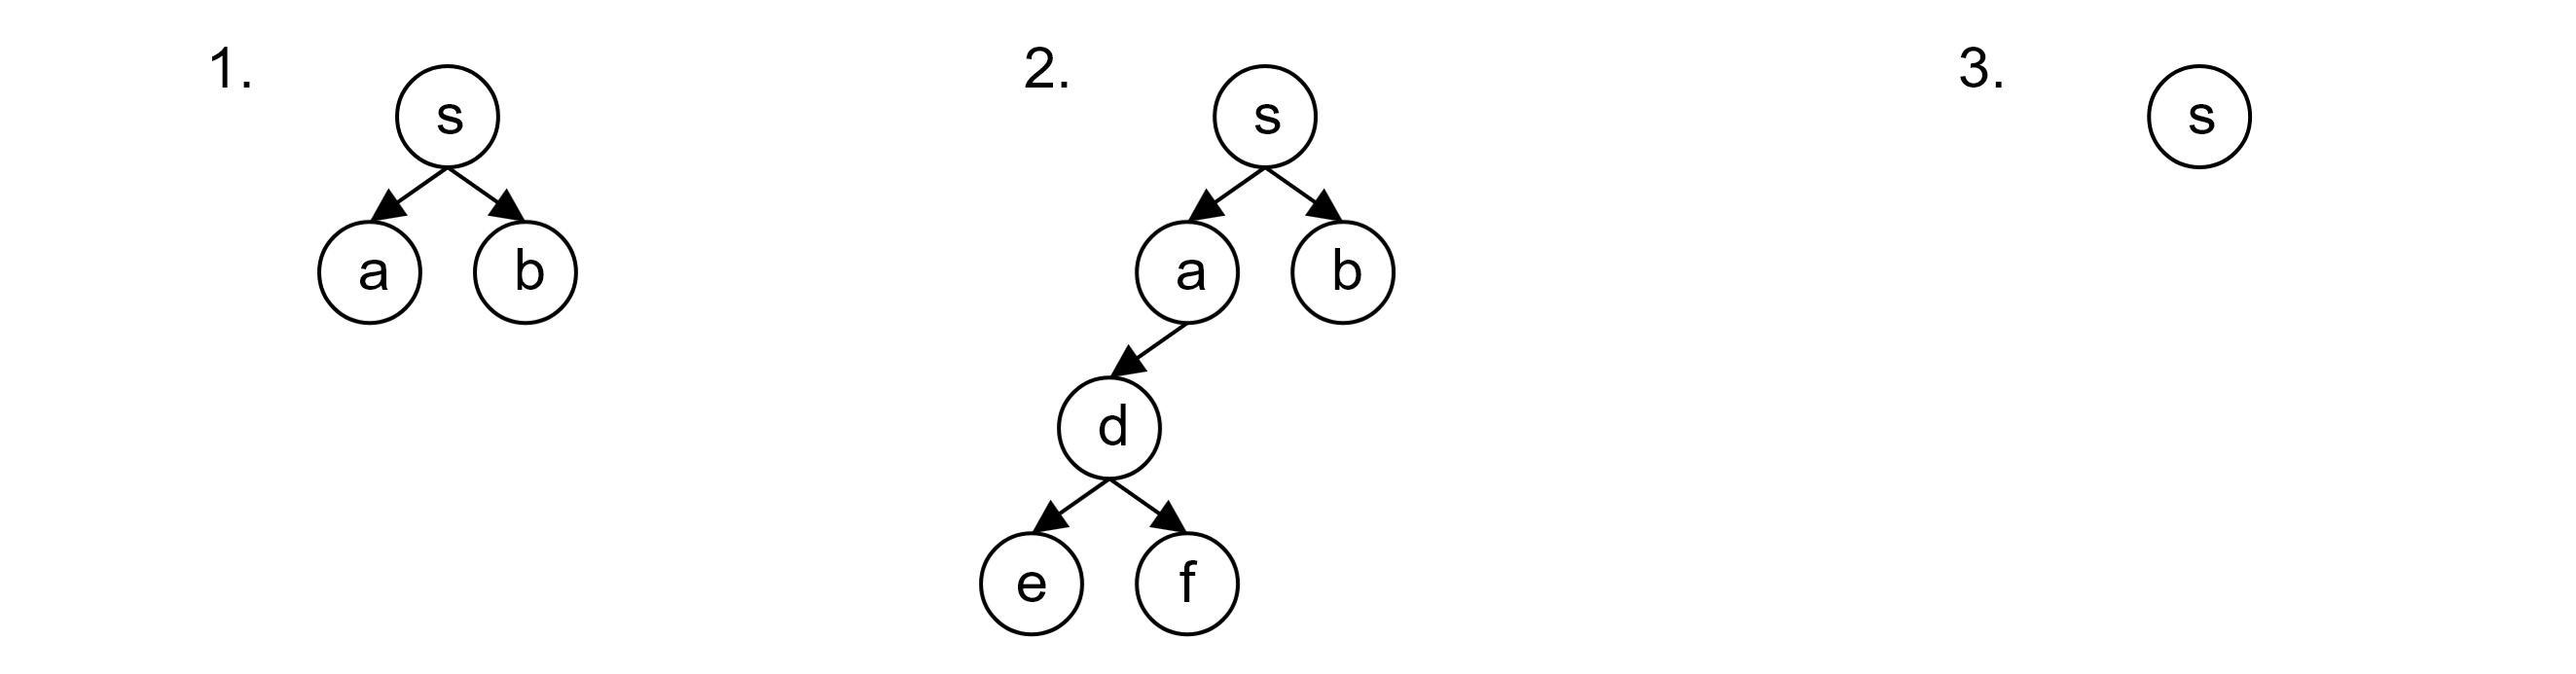
\includegraphics[width=\textwidth]{./Sections/graphs/binary_tree.png}
    \end{center}
     \caption{These are three examples of binary trees, including a single node (3).}\label{fig:binary_tree}
  \end{figure}

\noindent
To simply do a binary tree traversal, we may employ the following methods:
\begin{Func}[DFS Binary Tree Traversal - \texttt{DFS($T$)}]
    Depth-First Search on binary tree $T$ (recursive).
    
    \vspace{.5em}
    \noindent
    \textbf{Input:} Binary tree $T$.\\
    \textbf{Output:} Nodes in pre-order, in-order, and post-order.
    
    \begin{algorithm}[H]
        \SetAlgoLined
        \SetKwProg{Fn}{Function}{:}{}
        \Fn{\texttt{DFS($T$)}}{
            \If{$T$ is not empty}{
                Visit node $T$\;
                \texttt{DFS($T.left$)}\;
                \texttt{DFS($T.right$)}\;
            }
        }
    \end{algorithm}
    \noindent
    \rule{\textwidth}{0.4pt}
    \textbf{Time Complexity:} Given n nodes, and a force of a tree format, we have $n-1$ edges. Therefore with $m$ edges, $n+m = n+(n-1)$, hence $O(n)$ time.\\
    \textbf{Space Complexity:} again, we have $O(n)$ space for the stack.
\end{Func}

\noindent
$\mathbf{\rightarrow}$ \textbf{\underline{BFS has the same complexities} as per the same reasoning as the above function.}\\

\newpage
\noindent
The order in the above function is called \textbf{pre-order traversal};

\begin{Def}[Order Traversals]

    The order of traversal refers to the order in which nodes are visited/processed:
    \begin{itemize}
        \item \textbf{Pre-order:} Visit the node, then left, then right.
        \item \textbf{In-order:} Visit left, then the node, then right.
        \item \textbf{Post-order:} Visit left, then right, then the node.
    \end{itemize}
    In particular, \underline{\textbf{in-order traversal} is simply a run of \textbf{BFS}} as it processes the tree level by level starting 
    from the root.
\end{Def}

\noindent
Below is an example of all three:

\begin{Example}[Binary Tree Traversals (Part 1)]

    \begin{lstlisting}[language=Python, numbers=none]
    # Pre-order Traversal
    def PreOrder(T):
        if T is not None:
            visit(T)
            PreOrder(T.left)
            PreOrder(T.right)

    # In-order Traversal
    def InOrder(T):
        if T is not None:
            InOrder(T.left)
            visit(T)
            InOrder(T.right)

    # Post-order Traversal
    def PostOrder(T):
        if T is not None:
            PostOrder(T.left)
            PostOrder(T.right)
            visit(T)

    # Level-order Traversal
    def LevelOrder(T):
        BFS(T)
    \end{lstlisting}
\end{Example}

\newpage

\noindent
Now to show how this actually looks:
\begin{figure}[h]


    \hspace {-10em} 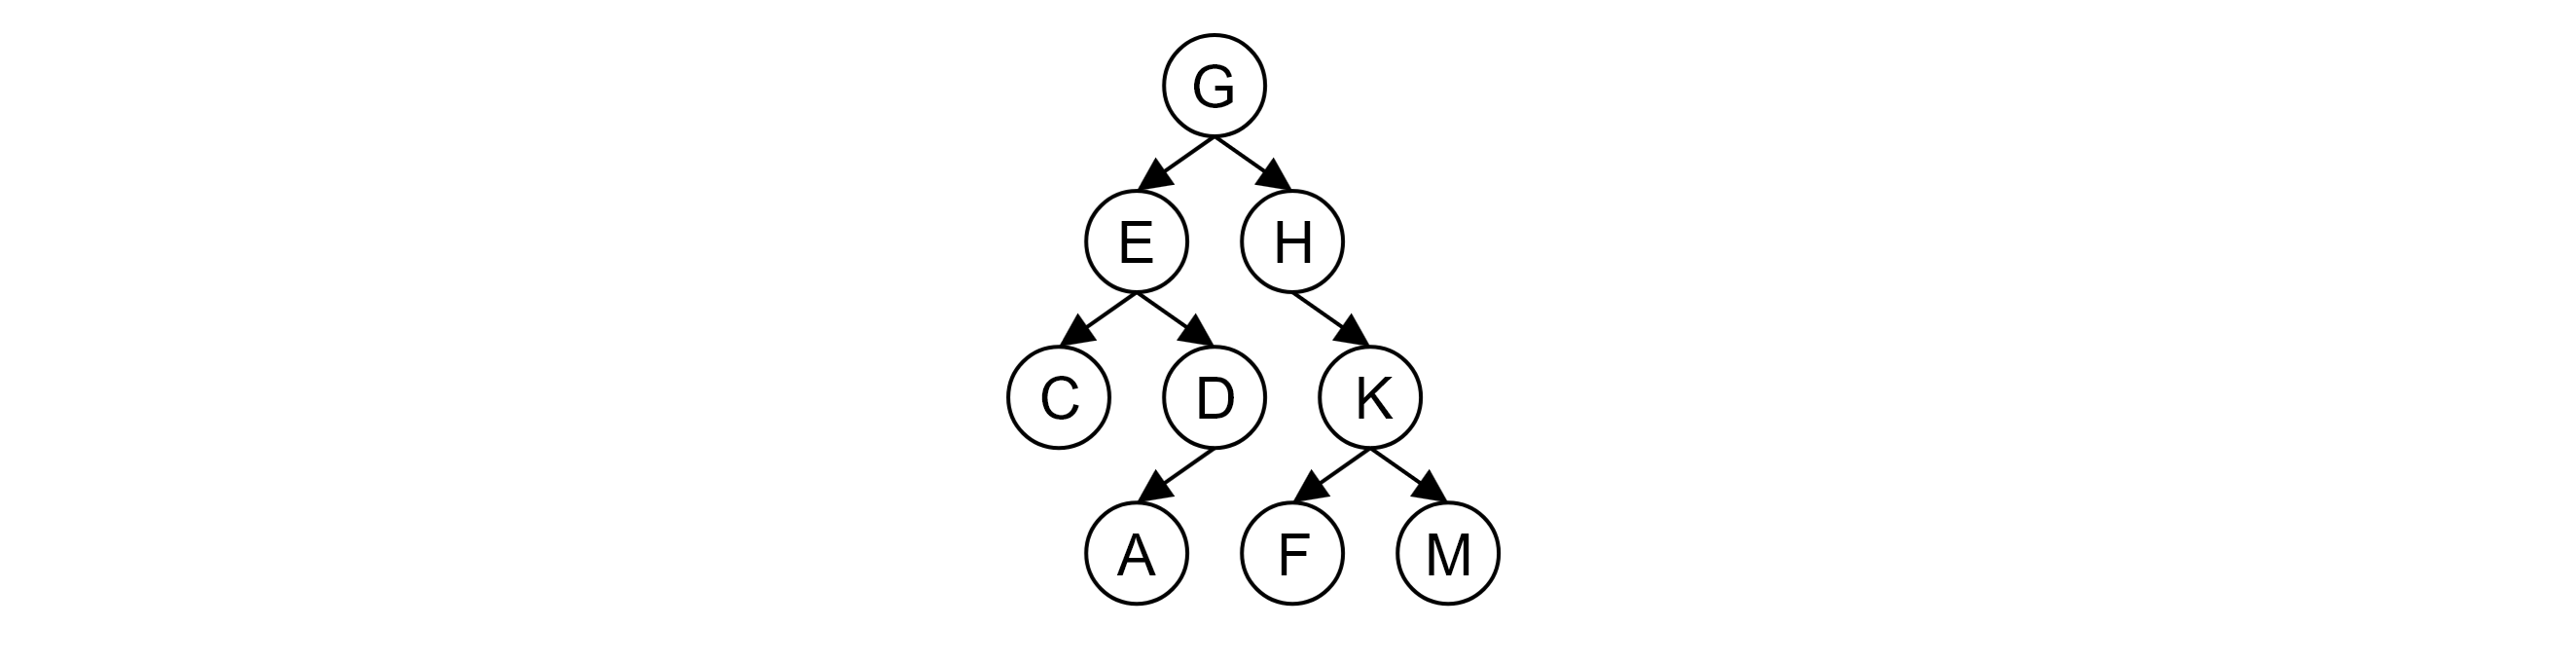
\includegraphics[width=1.5\textwidth]{./Sections/graphs/binary_tree_traversals.png}
  
     \caption{%
        The above binary tree has the following traversals:\\[1em]
           $\bullet$\quad  \textbf{Pre-order:}  \hspace{.5em} G, E, C, D, A, H, K, F, M\\
           $\bullet$\quad  \textbf{In-order:}   \hspace{1.2em} C, E, A, D, G, H, F, K, M\\
           $\bullet$\quad  \textbf{Post-order:} \hspace{.05em} C, A, D, E, F, M, K, H, G\\
           $\bullet$\quad \textbf{Level-order:} G, E, H, C, D, K, A, F, M\\[1em]
         Notably, if there is no left or right child to explore for that particular traversal order, that node then and there is processed.
     For example, in in-order traversal, since $C$ has no left child, it is processed first. The same goes for Post-order, where $D$ has no right child, so it is processed.
     }\label{fig:binary_tree_traversals}
  \end{figure}

\begin{Def}[Types of Binary Trees]

    There are several types of binary trees, each with its own properties:
    \begin{itemize}
        \item \textbf{Full Binary Tree:} Every node has either 0 or 2 children.
        \item \textbf{Complete Binary Tree:} All levels are fully filled except possibly the last level, which is filled from left to right.
        \item \textbf{Perfect Binary Tree:} All interior nodes have two children and all leaves are at the same level.
        \item \textbf{Balanced Binary Tree:} The height of the left and right subtrees of every node differ by at most one.
    \end{itemize}
    \noindent
    \textbf{Note:} A full binary tree is not necessarily complete, and a complete binary tree is not necessarily full.
\end{Def}

\newpage

\noindent
Observe the following examples of binary trees:
\begin{figure}[h]
    \begin{center}
    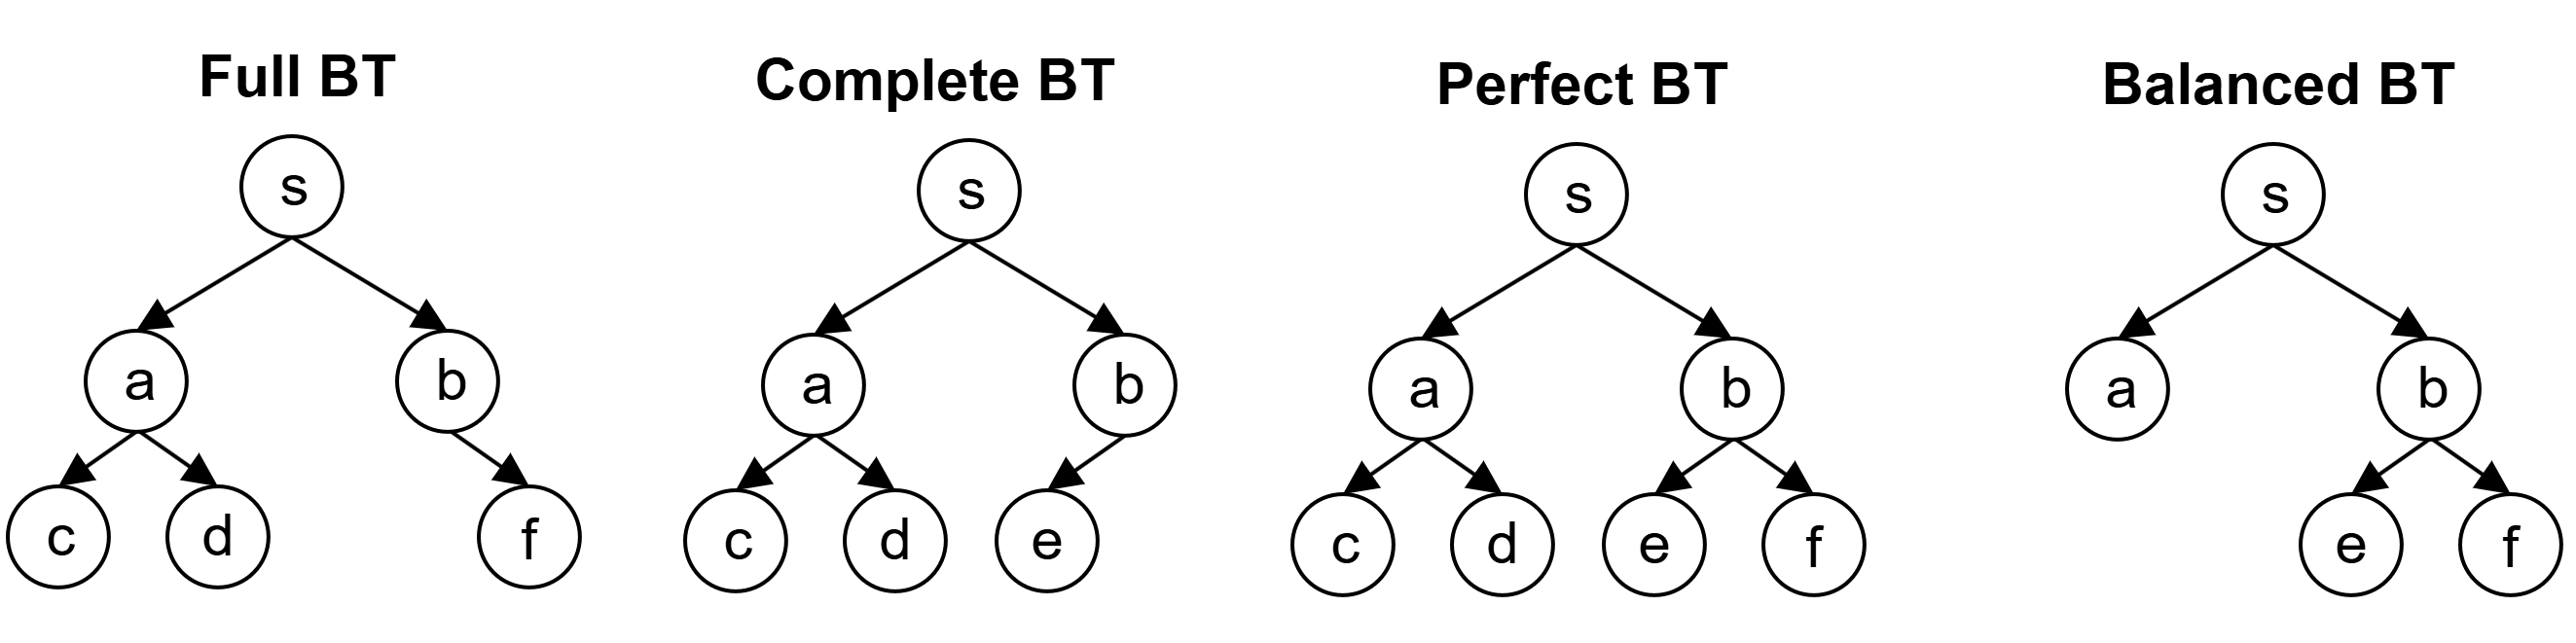
\includegraphics[width=\textwidth]{./Sections/graphs/search/binary_tree_types.png}
    \end{center}
     \caption{These are examples of different types of binary trees.}\label{fig:binary_tree_types}
  \end{figure}


\subsection{Binary Search Tree}
\noindent
A binary search tree is a stricter form of a binary tree, which gives us an efficient search algorithm.
\begin{Def}[Binary Search Tree (BST)]

    A \textbf{binary search tree} is a binary tree where:
    
    \begin{center}
        left child $<$ parent node $\leq$ right child
    \end{center}
    \noindent
    \textbf{Note:} A Binary Tree \underline{\textbf{is not}} a Binary Search Tree, unless it satisfies the above conditions.

\end{Def}
  \newpage 